% !TeX spellcheck = en_US

\addsection{Credits}{\images/experience.png}

\iftoggle{printable}{\vspace{-\baselineskip}}{}

\bigbreak

\begin{multicols*}{2}

This project shamelessly borrows best practices from the \href{https://github.com/Heegu-sama/Homm3BG}{\textbf{Rule Book Rewrite Project}}, including \LaTeX{} code, GitHub engineering, and translation framework.
You should check it out if you haven't seen it yet.

\textbf{Scenario templating, tooling and automation}: Andrzej Wiącek, Tomáš Zeman

\textbf{Contributing scenarios in \LaTeX{}:} Andrzej Wiącek, Tomáš Zeman, Xavier Borelly, Saveliy Ivanov, Tyson Heckert, Justus Törmälehto, Adam Obuchowicz, Vojtěch Růžička.  % no-check-caps

\phantom{Translators placeholder}

\textbf{Special thanks}: Patrick Kersten for \href{https://zedero.github.io/HoMM3BoardgameScenarioEditor/}{Scenario Map Editor}.
Everyone from Archon Studio, for producing the game and answering our incessant queries about rules and other topics.
Jon Van Caneghem and everyone involved with the development of the original video game.
Everyone who has supported the project with suggestions, corrections, image resources, and words of encouragement either on Discord or BoardGameGeek.

\textbf{Artwork borrowed from the official release was made by}: Tomasz Badalski, Yoann Boissonnet, Shen Fei, Viviane Tybusch Souza, Iana Vengerova, Bartosz Winkler

\columnbreak

\vspace*{\fill}

{\tikz[transparency group]\node[opacity=0.2]{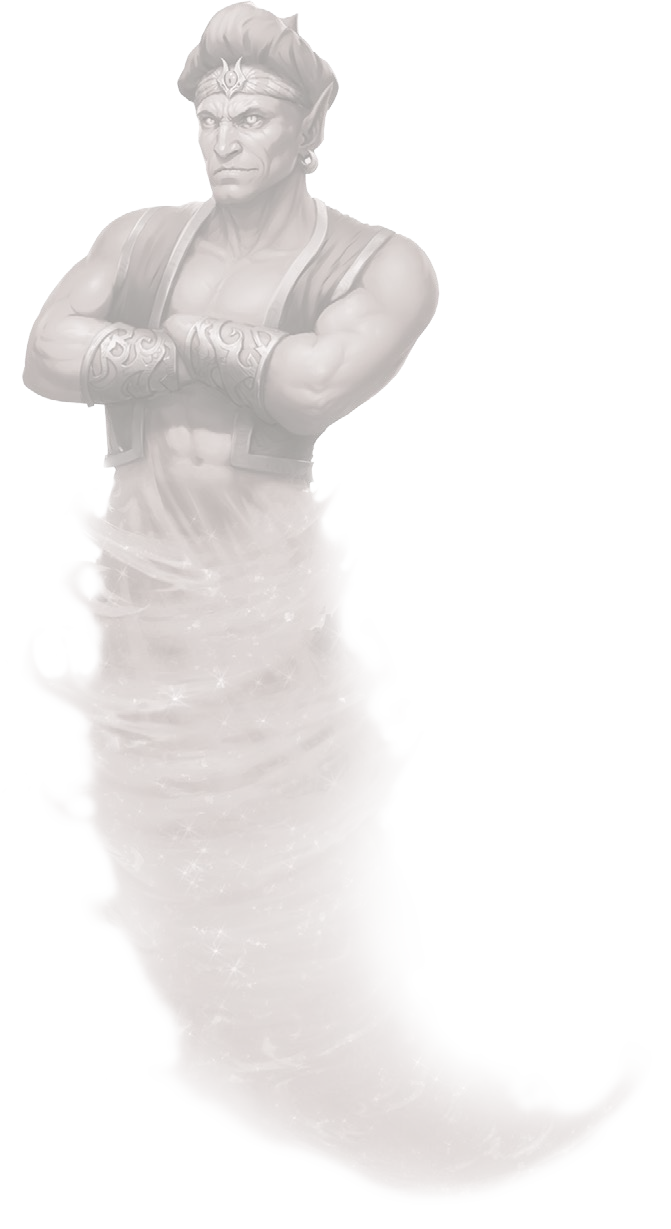
\includegraphics[width=1.3\linewidth]{\art/genie.png}};}

\vspace*{\fill}

\end{multicols*}
